\documentclass[a4paper,12pt,twoside,openright]{report}

\usepackage[pdfborder={0 0 0}]{hyperref}    % turns references into hyperlinks
\usepackage[margin=25mm]{geometry}  % adjusts page layout
\usepackage{graphicx}  % allows inclusion of PDF, PNG and JPG images
\usepackage{verbatim}
\usepackage{pdfpages}  % to embed proposal at the end of the dissertation
\usepackage{textcomp}
\usepackage{appendix}
\usepackage{subcaption}
\usepackage{tikz-uml}
\usepackage{csvsimple}

\usepackage{tikz} % Diagrams
\usetikzlibrary{positioning}
\definecolor {processblue}{cmyk}{0.96,0,0,0}

\renewcommand{\baselinestretch}{1.1}    % adjust line spacing

\begin{document}
	
	%%%%%%%%%%%%%%%%%%%%%%%%%%%%%%%%%%%%%%%%%%%%%%%%%%%%%%%%%%%%%%%%%%%%%%%%
	% Title
	
	
	\pagestyle{empty}
	
	\rightline{\LARGE \textbf{Peter Lotts}}
	
	\vspace*{60mm}
	\begin{center}
		\Huge
		\textbf{Adding network subsystem provenance collection to CADETS} \\[5mm]
		Computer Science Tripos -- Part II \\[5mm]
		Downing College \\[5mm]
		\today  % today's date
	\end{center}
	
	%%%%%%%%%%%%%%%%%%%%%%%%%%%%%%%%%%%%%%%%%%%%%%%%%%%%%%%%%%%%%%%%%%%%%%%%%%%%%%
	% Proforma, table of contents and list of figures
	
	\pagestyle{plain}
	
	\chapter*{Proforma}
	
	{\large
		\begin{tabular}{ll}
			Name:               & \bf Peter Lotts                       \\
			College:            & \bf Downing College                     \\
			Project Title:      & \bf Adding network subsystem provenance \\
								& \bf collection to CADETS \\
			Examination:        & \bf Computer Science Tripos -- Part II, 2018  \\
			Word Count:         & \bf 7493\footnotemark[1]  \\
			Project Originator: & Dr R.~Sohan                    \\
			Supervisor:         & Dr G.~Jenkinson                    \\ 
		\end{tabular}
	}
	\footnotetext[1]{This word count was computed on 12/05/2018	by \texttt{texcount -merge -dir -sub=chapter -utf8 -sum dissertation.tex}
	}
	\stepcounter{footnote}
	
	
	\section*{Original Aims of the Project}
	
	To provide additional metadata collection tools for network packets to the Computer Laboratory's existing CADETS project. This will be provided by tracking individual packets as they flow through the network stack of the FreeBSD\footnote{\texttt{http://www.freebsd.org/}} kernel, and making information regarding memory locations used and the time taken by each layer to process a given packet available to DTrace\footnote{\texttt{http://dtrace.org/}}. DTrace is a generic Dynamic Tracing framework which is the primary data collection tool used by the CADETS project to bring kernel data into userspace for analysis. The performance impact of the project on network packet delivery is to be evaluated.
	
	
	\section*{Work Completed}
	
	I have implemented a scheme for assigning Universally Unique Identifiers to each packet passing through the network stack of the FreeBSD kernel, along with DTrace probes to extract information pertaining to the now-identifiable packets. I extract this information in an example user-space application which stores the data it receives in memory and is able to provide aggregated data, graphs etc. to users via a Web front end.
	
	\section*{Special Difficulties}
	
	None.
	
	\newpage
	\section*{Declaration Of Originality}
	
	I, Peter Lotts of Downing College, being a candidate for Part II of
	the Computer Science Tripos, hereby declare
	that this dissertation and the work described in it are my own work,
	unaided except as may be specified below, and that the dissertation
	does not contain material that has already been used to any substantial
	extent for a comparable purpose.
	
	\bigskip
	\leftline{Signed [signature]}
	
	\medskip
	\leftline{Date [date]}
	
	\tableofcontents
	
	\listoffigures
	
	%%%%%%%%%%%%%%%%%%%%%%%%%%%%%%%%%%%%%%%%%%%%%%%%%%%%%%%%%%%%%%%%%%%%%%%
	% now for the chapters
	
	\pagestyle{headings}
	
	\chapter{Introduction}
	
	\section{Use Case}
	
	In this project I am evaluating the application of fine-grained tracing within the network stack of the FreeBSD kernel by implementing additional statically defined DTrace probes which are able to provide a platform for both security and performance analysis.
	
	The security aspect of the tool is most useful in combating Advanced Persistent Threats (APTs)\cite{Tankard-APT}, where the attacker slowly infiltrates the target system, hiding out of sight until they can exploit knowledge gained to access the enterprise’s internal network. This may allow the attacker to extract sensitive data, from databases for example, in such a way that the access is very hard to distinguish from normal access. Eventually, it is likely that the malware will make a mistake and trigger an indicator of compromise to be observed by administrators, but by then it is difficult to tell what data the malware has seen.
	
	As pat of the DARPA Transparent Computing Program\cite{DARPA-CT}, the Computer Laboratory has a project which is trying to combat this by building CADETS\cite{CADETS-main} on top of the FreeBSD operating system, which tracks the provenance of data by collecting metadata from computers all over the network about what processes act on what data and when. This metadata is then collected in a distributed database, where it can be analysed to trace data flows throughout the computer system.
	
	My project adds support for collecting metadata on network packets as they flow through the kernel	network stack. The data collected will allow users of CADETS to seek out suspicious activity which may be being used to attack a system, and will be able to provide a list of locations in kernel memory where packet data were stored. The latter allows a system administrator to infer what data may have been leaked if they are able to determine that some malicious code had access to a particular set of kernel memory addresses.
	
	The performance analysis platform is provided by DTrace's provision of high-accuracy timestamps on probe firing, which when they are collated for a given packet allow the time spent in each section of the network stack to be evaluated. This could be assessed by system administrators, and may allow for better fine-tuning of protocol parameters, some of which are notoriously difficult to set.
	
	\section{The Network Stack}
	
	Almost all modern general purpose computer networks (including, significantly, the Internet) are built upon a layering of several protocols on top of each-other with well-defined interfaces connecting them, defined by the OSI model\cite{ISO-OSI}. These interfaces are often quite general and so this model allows for different protocols to be used for each layer as desired, somewhat interchangeably; this also provides code separation between modules (i.e. layers) with different duties, and so make implementations of these layers - the so-called `Network Stack' - easier to maintain.
	
	\subsection{Layer 1: Physical}
	The bottom-most layer of the network stack, this layer defines the physical communications medium and how to transmit bit streams over it. Properties such as timing, leading to latency and bandwidth, are mostly defined in this layer, although higher layers are likely to decrease bandwidth somewhat by adding mandatory per-packet header data. Generally these days this layer is 802.11 (`Wi-Fi') or Ethernet, although Ethernet networks generally do not need to handle shared medium communications any more.
	
	\subsection{Layer 2: Data Link}
	This layer defines how data frames are transferred between two physically connected nodes, including any shared medium access arbitration and means of addressing such physically connected nodes.
	
	\subsection{Layer 3: Network}
	Typically implemented by the Internet Protocol (IP), addressing and routing between physical networks is defined here, typically including concepts such as broadcast (all nodes receive message) and multicast (a specific group of nodes receive message). This layer often has to handle problems arising from the underlying layers having a different Maximum Transmission Unit (MTU), such that a large packet may not be able to make the next hop in the path as a single packet if it is too large for the next physical network. In IPv4 this is handled using fragmentation, where the large packet is split up into several smaller ones which are then sent separately, and the receiver must keep a copy of fragments it receives until it can re-assemble the whole packet and deliver it to the layer above. IPv6 addresses the problem by dropping the packet and sending a notification back to the sender. Fragmentation is not, however, a common process, with some empirical studies showing that the rate of fragmentation in the open internet is as low as 0.25\%.
	
	\subsection{Layer 4: Transport}
	This layer is responsible for the reliable delivery of data (if required) across a layer 3 link, and creates the notion of a connection which is opened, used to transmit/receive data, and then closed. This is the most common place for application designers to make a choice about layer implementation - TCP or UDP. TCP (the Transmission Control Protocol) provides reliable, in-order delivery of data to higher layers, along with trying to provide fairness between connections through adaptive transmission rate control to avoid congestion. Its main alternative, UDP (the User Datagram Protocol), does not provide reliable delivery but in removing this feature is often able to operate with lower latency than TCP.
	
	\subsection{UNIX Sockets API}
	Under the UNIX `everything is a file' abstraction, layer 4 connections are provided to user applications through sockets, objects which are opened and closed in a similar manner to files and which yield a file descriptor for I/O operations while the connection is open. This abstraction is provided by the kernel (meaning all layers described previously are implemented either in hardware or the kernel) and used by other kernel components as well as all userspace applications which perform network communication.
	
	\section{Probe Effect}	
	When tracing any application, it is important to consider the performance impact of the tracing system on the target application. Timings can be critical to correct operation of the application, but even when this is not the case it would still be all too easy to impact system performance to the point where it no longer meets specifications. Causing the system to degrade to this point undermines the purpose of the tracing in the first place - namely to run all the time the application is running in the real world to gather data which is later used for security and performance analysis.
	
	Of all applications, it is of the utmost importance not to slow down the operation of the Operating System kernel beyond what is necessary. Every application running on the computer must interact with the kernel to perform I/O to files, networks and so forth, and so slowing down the kernel will impact on all applications which use it. This is especially true of regions which operate under mutual exclusion and so the usual modern-day approach of shifting to multicore may not be able to help.
	
	With regards to timings affecting system operation, parts of the network stack are particularly vulnerable to latency, as timers are integral to their operation. One example of such a protocol is TCP, where Padhye\cite{Padhye-TCP} has shown that the throughput of a TCP connection is inversely proportional to the latency which TCP observes on the network connection. Clearly, any undue addition to this latency by low-level network code could have dire consequences for application throughput on the system.
	
	\section{Similar Work}
	
	Fonseca et al.\cite{X-Trace} describes X-Trace, which provides a similar solution to my project but only for user level applications; it attaches metadata to the real data flow within the application, and then traps this prior to data transmission and logs the metadata using a separate system. While my project will be attaching metadata to kernel packets, it will not be collecting metadata together in the kernel, instead firing a DTrace probe for each event.
	
	The X-Trace website itself says that it has largely been superseded by another tool, Pivot Tracing, presented by Mace\cite{Pivot-Tracing}. Pivot Tracing focusses on analysing event data by using a `happens-before join' operator when aggregating data across machines on a network, and so is more comparable the existing CADETS code base rather than the code being added by this project.
	
	Under Linux, the Resourceful\cite{Resourceful} framework is able to collect data from auto-generated tracepoints	within the Linux kernel with very low overhead by modifying the kernel code on the fly on the running system, but Resourceful does not currently inspect the network subsystem at all.
	
	\section{Overall design}
	
	The project is to assign uniquely identifying tags to each packet as it flows through the network stack, noting that packet fragmentation/reassembly will make this more difficult. This will then allow DTrace tracepoints to read the tag on each packet when an interesting operation (broadly speaking, a memory allocation) is performed on it. From here, scripts written in DTrace's D language will be able to forward information to a DTrace consumer to display results and answer user queries.

	
	
	\chapter{Preparation}
	
	\section{Starting Point}
	\label{sec:starting-point}
	
	The CADETS project currently has a user-space application which collects metadata on kernel-level	datastructures via libdtrace, translates the metadata to a JSON format for easy interpretation, and	then sends this away for processing (often over the network). It also has an application with a user interface to display the data it has collected.
	
	The FreeBSD kernel provides a means of tagging its main internal structure of interest, namely \verb|struct mbuf| using \verb|struct mbuf_tags|. It is thought that this will be sufficient to tag a packet’s data with an unique identifier in order to track its progress through the kernel’s network stack. \verb|struct mbuf| is used by the FreeBSD kernel as a generic fixed size memory buffer (hence the name) to store network packet data as it passes from the sockets API all the way to physical network interfaces. The structures have the ability to be chained together in a linked-list like structure to store variable amounts of data, and packets are edited in place where headers must be added and so forth.
	
	Under Linux, the Resourceful framework is able to collect data from auto-generated tracepoints	within the Linux kernel with relatively low overhead, but it does not currently inspect the network subsystem.
	
	\section{Installing the Development System}
	
	I had no prior experience with FreeBSD usage or development, so the first challenge was to get a system up and running to be used for both development and testing. I decided to host FreeBSD as a virtual machine on my Windows 10 laptop, as it has reasonable performance for compiling code, whilst being portable and allowing me to work on the project wherever I am. The virtual machine was set up using Oracle\texttrademark\ VM VirtualBox\footnote{\texttt{http://www.virtualbox.org/}}, as I have most experience using this virtualisation application.
	
	The FreeBSD website provides preinstalled images\footnote{\texttt{http://www.freebsd.org/where.html\#download}} for various virtual machine types, and I decided to use one of these as a basis due to my inexperience with the operating system. Only slow progress was made during the first few days of using this new operating system, as the preinstalled images have a rather basic toolset available and I had to learn how to use a new package manager, and the FreeBSD `ports' system. Having acclimatised to these, I was able to fork the CADETS custom kernel, build and install it onto the running machine.
	
	\section{FreeBSD kernel study}
	
	The first significant piece of planned project work was to inspect the FreeBSD kernel source code for the network stack, gain some familiarity with it, and note the locations of operations which are of particular interest to the project, either from a packet tagging perspective or from the perspective of packet data being copied to a new memory location.
	
	The study commenced at the point where outgoing packets enter the IP layer of the network stack, namely the top of the \verb|ip_output| function. From here, the packet was followed down through the IP layer, exploring all possible control paths
	\footnote{
		With one or two notable exceptions, namely that
		\begin{itemize}
			\item Berkley Packet Filter (BPF) was considered to be out of scope for the project
			\item IPSec allows arbitrary code to be executed via its `hooks' system, and so this cannot be inspected
		\end{itemize}
	}
	and possible exit routes into lower layers. Once the packets had left to go to device drivers, the study then turned to the \texttt{netisr} system, which is responsible for receiving packets from device drivers in the FreeBSD kernel and handing them on to the appropriate next layer (usually the IP layer) to be processed. From here, packets were followed back up the network stack in a similar manner, up to the end of \verb|ip_input|, where packets leave the IP layer to go to the next layer up.
	
	At this point, it was noticed that the project was getting a little behind schedule and, in a meeting with my supervisor, it was decided that for the moment the project would not look any higher than the IP layer, as there was no significant academic benefit to be gained from continuing up to look at the TCP layer\footnote{In order to associate packets with sockets, however, a small amount of tracing would have to be added to the TCP layer.}. This could be completed at a later stage in the project if time became available.
	
	\section{Challenges of kernel development}
	
	It is generally accepted that kernel development is more difficult than application level development, and that productivity is lower as a result. This is in part due to the language choices involved - the FreeBSD kernel is written in C and there is no way to change that whereas in application code it is possible to use the most appropriate language for the job at hand; at least as high level as C++, anyway. Kernel APIs tend to have more opaque documentation as the focus is on documenting the exact specifications of a call, rather than getting people to use it quickly. Internet searches are often less productive as fewer people have ever encountered your exact situation before, and of course extra care must be taken to understand every line of code written, as any memory access error will result in the kernel panicking - and it is much harder to debug the kernel than it is to debug a userspace application.
	
	Although I had experience in C/C++ prior to starting this project, I had no experience with the FreeBSD operating system from either a user's perspective or a developer's. I had occasionally compiled the Linux kernel, but had only done any work on it far enough to fix compile errors. Given this situation, reading through the kernel source code was a non-trivial exercise, as I was not familiar with any of the kernel data structures in use and so had to research these when I encountered them. The pain of doing this is greatly reduced by the existence of M.K. McKusick et al's book, `The Design and Implementation of the FreeBSD Operating System'\cite{McKusick:2014:DIF:2659919}, and Robert Watson's FreeBSD Kernel Cross-Reference\footnote{http://fxr.watson.org/}, which allows one to search for identifiers throughout the kernel source tree. It does not compare to some modern IDEs for development, but as these were not readily available on my development machine the online system was sufficient.
	
	\section{Requirements Analysis}
	
	\subsection{Kernel portion}
	
	The project must provide means of uniquely identifying packets in the network stack of the operating system and associating these identities with timing information and memory addresses used to store data. This is to be moved from kernel space to user space using DTrace, as this will allow the data collection to be integrated with the wider CADETS system if required, as well as other applications in the future.
	
	\subsection{Userspace application}
	
	To demonstrate the power of the kernel-level tool which has been produced, the project will also provide an example application to collect and analyse the data produced by the kernel, which is extension 1 in the project proposal. This application shall consist of three main components; data input takes the form of a DTrace consumer which uses libdtrace to enable probes and gather data, data storage uses carefully considered data structures in order to balance the trade-off between memory space consumed and access performance, and analysis is performed by the final component, which displays its results through a Web-based front-end. I chose such a front-end because I did not feel that spending project time getting a graphical user interface up and running on FreeBSD had any academic value, and a Web tool provides accessibility for system administrators who would wish to use this application on headless servers.
	
	\section{UUID algorithm selection}
	
	As I have discussed earlier, a key part of the kernel development will be to minimise the impact which additional tracing code has on the performance of the network stack, in particular latency and throughput. The algorithm used to generate unique identifiers is expected to be the most costly operation added to the kernel, so this should be chosen with care. In principle it is possible to reduce the cost of UUID generation to this project by adding an additional piece of hardware to the computer, perhaps made available by the kernel through the /dev interface, to continuously generate a pool of UUIDs. However, for this project I have decided not to use such a system so that my code can be used on systems without such external hardware.
	
	Although it is expected that the generation of UUIDs will be the most costly operation involved in packet tagging, it is also possible that storing UUIDs for each packet will have a significant impact on performance on the network stack. It has been shown that \verb|mbuf|s which are poorly aligned for the local cache architecture can have such an impact, and a similar issue could be caused if the UUID storage shares a cache line with part of an \verb|mbuf|, and so increases cache pressure on the system.
	
	\subsection{Available algorithms}
	
	The rest of CADETS is already using Universally Unique Identifiers (UUIDs) in other parts of the system, so it would be sensible to use these for packets as well. UUIDs are standardised by RFC4122\cite{RFC4122}, with the two candidates here being version 1 (described in section 4.2) and version 5 (section 4.3), both of which have already been implemented in the CADETS fork of the FreeBSD kernel. The output of the two algorithms is syntactically the same, namely a 128-bit value, but they differ semantically. UUIDv1 uses the current time (considered to be a non-decreasing function) and the computer's MAC address (relatively unique, certainly should be unique within the network) to generate unique identifiers. UUIDv5, on the other hand, takes its uniqueness from a unique name within some arbitrary namespace which is passed to it, and then constrains the output to a fixed length by using a SHA-1 hash.
	
	\subsection{Benchmarking}
	
	To inform the choice of algorithm, I decided to compare the expected performance of the network stack when tagging packets with each form of UUID. I estimated this performance by inserting a single call to the desired generation algorithm at the beginning of the \verb|ip_output| function, as this would cause the function to be called once for each IP layer packet sent out of the system.
	
	Details of the benchmark and experimental method used are provided in Section \ref{sec:IPC-expt}; it suffices to say at this point that the benchmark provides an estimate of the maximum possible throughput through the (virtualised) loopback network adapter.
	
	\subsection{Results}
	
	\begin{figure}
		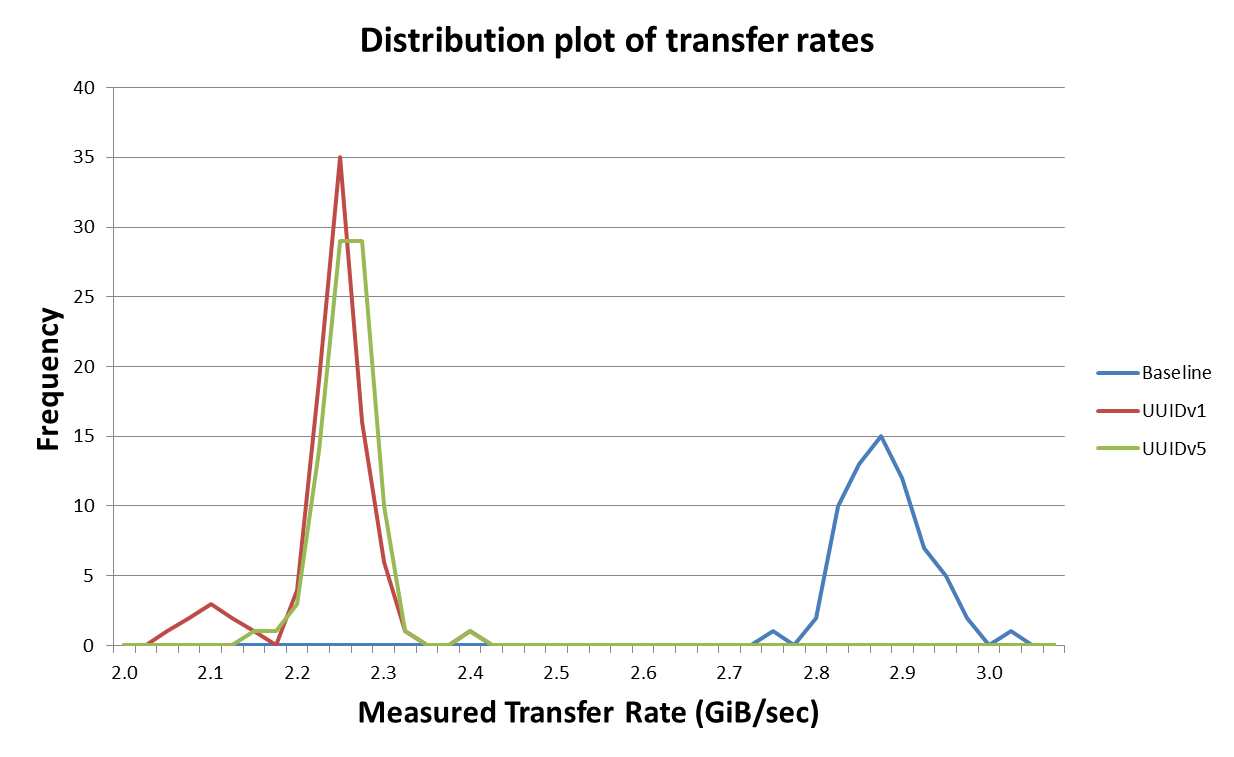
\includegraphics[width=\linewidth]{include/IPC-uuid-bench.png}
		\caption{Plot of the distribution of throughput values for each UUID generator. The shape of all 3 distributions is broadly similar, as would be expected, with an equal performance drop for both UUIDv1 and UUIDv5.}
		\label{fig:IPC-uuid-bench}
	\end{figure}
	
	As shown in \figurename{\ref{fig:IPC-uuid-bench}}, the addition of UUID a generation algorithm did have a negative impact on performance, with a 20\% reduction in performance for both algorithms. There is little difference between the speed of the two algorithms, which is particularly surprising given how different they are in modus operandi.
	
	\subsection{Conclusion}
	
	From the results in \figurename{\ref{fig:IPC-uuid-bench}}, there is clearly little to pick between the two UUID generation algorithms under consideration. However, this test was run with constant inputs to the v5 generator, and so the v5 system would still need some way of generating unique inputs. Doing so would likely involve implementing something similar to the v1 algorithm in our case, and so I chose to proceed using version 1 of the algorithm.
	
	
	\chapter{Implementation}
	
	\section{Kernel alterations}
	
	\subsection{Tagging packets with UUIDs}
	
	As discussed in Section \ref{sec:starting-point}, the FreeBSD kernel provides \verb|struct mbuf_tags| to attach arbitrary tags to packets (which are stored in \verb|struct mbuf|). In order to make use of this facility, I had to declare a new \verb|struct|, containing the \verb|mbuf_tags| structure alongside the data I actually wanted to store. Other basic setup is also required to use the new \verb|struct| - a numeric constant (`cookie') must be defined so that the new tag can be recognised (since C does not provide reflection), and a further constant must be defined in order to be able to allocate the new structure using the kernel version of \verb|malloc()|. Only once all this setup was complete could I use the new \verb|struct mtag_uuid|.
	
	The overriding design goal for this new kernel component was to provide a clear, concise interface to the rest of the kernel, ideally only requiring a single function call to be inserted at a given point in other files. All functions have been declared to begin with the prefix \verb|net_uuid| (also the name of the component as a whole) in order to prevent namespace pollution for existing code and to make it clear when control flows into this component. A single call to \verb|net_uuid_tag_packet()| at the point a packet enters the scope of tracing will generate a UUID for the packet and attach a new tag to it. The names of the \verb|net_uuid_*| family of functions are quite long by kernel standards so as to be transparent about what each function does.
	
	Reflecting the code's place in the operating system kernel, I have used the defensive programming technique on all the functions defined by the external interface (and most internal ones) in order to ensure that sensible behaviour occurs when functions receive a NULL, or otherwise invalid, argument. As this code is only for tracing such scenarios do not represent errors for the system as a whole, so are mostly ignored silently. I used defensive programming to provide graceful degradation in the event of a failure in my code, so that for example the kernel does not crash due to a memory error - in all cases, it is considered safer to not trace a particular packet than crash the kernel.
	
	The \verb|struct mtag_uuid|, as shown in \figurename{ \ref{fig:mtag_uuid}}, also contains pointers to other structures which together allow a tree of such tags to be formed, representing the fragmentation and reassembly of packets which may occur in the network stack. This adds complication when it comes to freeing the structure, as it would not be acceptable for kernel code to cause memory leaks and so the whole tree must be freed carefully. To do this, the free function uses a linked list as a queue in order to perform a breadth-first search of all tags in the tree. The FreeBSD kernel makes available a set of macros for the management of linked lists, as of course the C standard does not contain such advanced data structures.
	
	\begin{figure}
		\begin{verbatim}
		struct mtag_uuid {
		    struct m_tag       tag;
		    struct uuid        uuid;
		    struct mtag_uuid  *parent;
		    struct mtag_uuid  *child;
		    struct mtag_uuid  *sibling;
		    void             (*m_free_tag_default)(struct m_tag *);
		};
		\end{verbatim}
		\caption{The declaration of the packet tag structure. The required mtag structure comes first in memory, followed by the UUID and tree pointers.}
		\label{fig:mtag_uuid}
	\end{figure}
	
	\subsection{Adding a kernel configuration option}
	
	As this code is likely to impact the performance of the network stack, and it is only useful when used in conjunction with a DTrace consumer, I felt it was important to provide a kernel configuration option to disable the additional code for this component. All I had to do for this was to declare the option in \verb|sys/conf/options| within the kernel source tree, and provide documentation in \verb|NOTES| in the same directory. Following inclusion of a special header file generated by the build system, my code simply had to check for a C preprocessor definition and, if present, it defines all the \verb|net_uuid_*| functions to do nothing - it is very likely that the compiler will then optimise these calls out completely.
	
	\subsection{DTrace probes}
	
	DTrace probes can be part of any one of several `providers', depending on how they are defined. In this project I am using the Statically Defined Tracing (SDT) provider to set fixed probe points within the kernel code. All work with these probes is done using preprocessor macros defined by the SDT provider to fill everything in for me. I first had to declare and define (in a header and source file, respectively) the different probes I would be using, and then these probes are used with further macros. In the same style as the TCP and IP subsystems', I decided to provide shortened macros (all named \verb|NET_UUID_*| for similar reasons to previously) to fire the probes which I would be creating.
	
	Due to limitations within DTrace's D language, the probes currently involve more work in the kernel than would be ideal. The process of locating the required tag on an mbuf and extracting the UUID from this must be performed before the probe is fired, as DTrace is unable to do this. In other areas, however, DTrace has some nice features which are advantageous here, including the concept of type translations between native kernel types and special types in the D language. These are used to provide a stable type in DTrace for a particular probe, even when the underlying kernel type may be altered.
	
	\section{The red-black ternary search tree}
	\label{sec:TST-impl}
	
	\begin{figure}
		\begin{subfigure}{\textwidth}
			\centering
			\begin {tikzpicture}[-latex, auto, semithick,
			trienode/.style = {
				rectangle, top color = white, bottom color = processblue!20, draw, processblue, text=blue, minimum height = 13mm, minimum width = 37mm
			},
			trieptr/.style = {
				rectangle, draw=black!50, minimum width = 3mm, minimum height = 5mm, anchor=south west
			}
			]
			
			\newcommand{\drawtrienode}[3]{
				\node[trienode] (#1) 	at #2{};
				\node[anchor=north west] at (#1.north west) {Leaf: #3};
				\node[trieptr]  (#1-0)	[above = of #1.south west, yshift = -8mm, xshift=4mm]{};
				
				\foreach \i in {1,...,9}
				{
					\pgfmathtruncatemacro{\j}{\i - 1};
					\node[trieptr] (#1-\i) at (#1-\j.south east) {};
				}
			}
			
			\drawtrienode{root}{(0, 0)}{false}
			
			\drawtrienode{2}{( -3, -3)}{true}
			\drawtrienode{5}{(  0, -5)}{false}
			\drawtrienode{9}{(  4, -3)}{false}
			
			\drawtrienode{26}{( -5, -6)}{true}
			\drawtrienode{27}{( -3, -8)}{true}
			\drawtrienode{53}{( -1,-10)}{true}
			\drawtrienode{90}{(2.5, -7)}{true}
			\drawtrienode{94}{(  7, -7)}{true}
			
			\drawtrienode{902}{(  4,-10)}{true}
			
			
			\path (root-2) edge node {2} (2);
			\path (root-5) edge node {5} (5);
			\path (root-9) edge node {9} (9);
			
			\path (2-6) edge node {6} (26);
			\path (2-7) edge node {7} (27);
			\path (5-3) edge node {3} (53);
			\path (9-0) edge node {0} (90);
			\path (9-4) edge node {4} (94);
			
			\path (90-2) edge node {2} (902);
			
		\end{tikzpicture}
		\caption{Array-based trie representation}
		\end{subfigure}
		\par\bigskip\bigskip
		\begin{subfigure}{\linewidth}
			\centering
			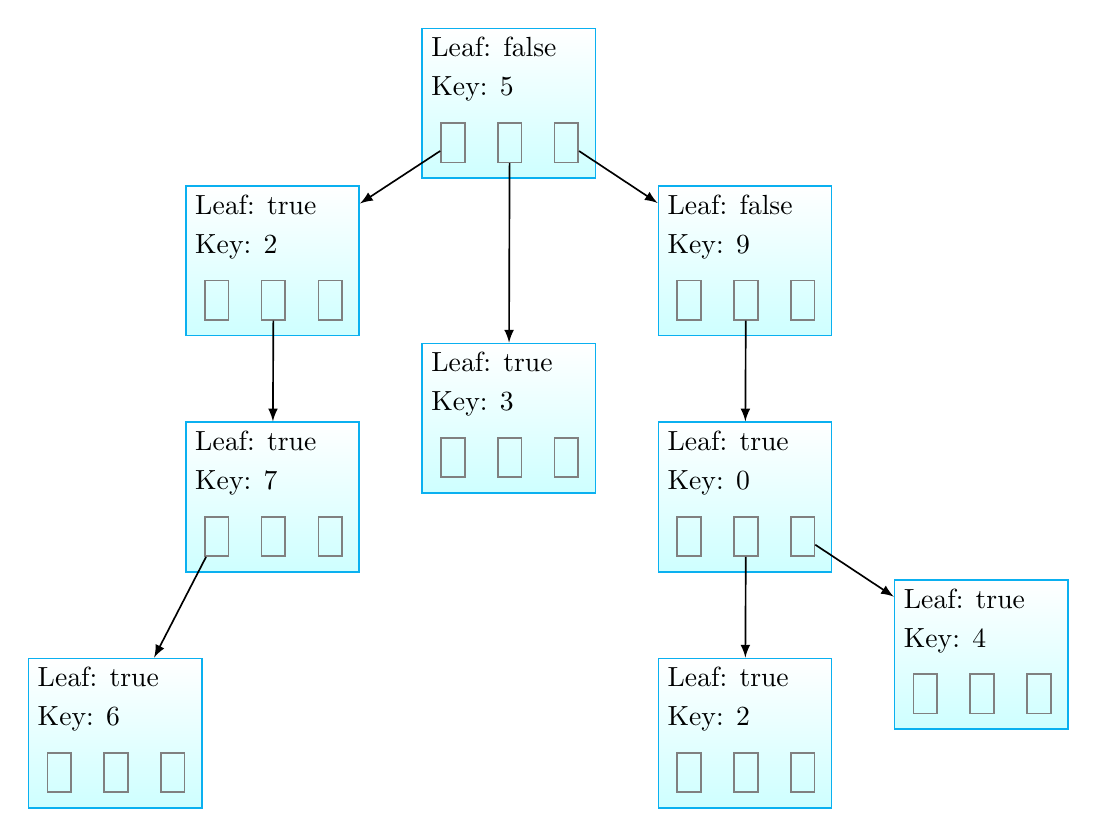
\begin{tikzpicture}[-latex, auto, semithick,
			tstnode/.style = {
				rectangle, top color = white, bottom color = processblue!20, draw, processblue, text=blue, minimum height = 19mm, minimum width = 22mm
			},
			trieptr/.style = {
				rectangle, draw=black!50, minimum width = 3mm, minimum height = 5mm, anchor=south west
			}
			]
			
			\newcommand{\drawtstnode}[4]{
				\node[tstnode] (#1) 	at #2{};
				\node[anchor=north west] (#1-lf) at (#1.north west) {Leaf: #4};
				\node[anchor=north west] at (#1-lf.south west) {Key: #3};
				\node[trieptr]  (#1-left)	[above = of #1.south west, yshift = -8mm, xshift=4mm]{};
				\node[trieptr] (#1-mid) at (#1-left.south east) [xshift=4mm] {};
				\node[trieptr] (#1-right) at (#1-mid.south east) [xshift=4mm] {};
			}
			
			\drawtstnode{5}{(  0,  0)}{5}{false}
			\drawtstnode{2}{( -3, -2)}{2}{true}
			\drawtstnode{9}{(  3, -2)}{9}{false}
			
			\drawtstnode{27}{( -3, -5)}{7}{true}
			\drawtstnode{26}{( -5, -8)}{6}{true}
			\drawtstnode{53}{(  0, -4)}{3}{true}
			\drawtstnode{90}{(  3, -5)}{0}{true}
			\drawtstnode{94}{(  6, -7)}{4}{true}
			
			\drawtstnode{902}{( 3, -8)}{2}{true}
			
			\path (5-left) edge node {} (2);
			\path (5-mid) edge node {} (53);
			\path (5-right) edge node {} (9);
			\path (2-mid) edge node {} (27);
			\path (9-mid) edge node {} (90);
			
			\path (27-left) edge node {} (26);
			\path (90-mid) edge node {} (902);
			\path (90-right) edge node {} (94);
			
			\end{tikzpicture}
			\caption{Ternary Search Tree representation}
		\end{subfigure}
		\caption{A traditional array-based trie structure whose alphabet is the integers 0-9 (a), and a corresponding TST (b). These structures both contain the strings 2, 26, 27, 53, 90, 902, 94. Characters on pointer edges are shown for clarity only.}
		\label{fig:trie-tst}
	\end{figure}
	
	\subsection{Motivation}
	
	In this project, I needed a data structure to form a map of (generally string) keys to values, usually pointers to a data structure holding information about a particular packet. It is also important to the end application that the data structure be able to search within a key prefix in order to provide, for example, information on a particular chunk of memory address space, characterised by the high bits of its address. There are various ways to implement a key-value store of this type, including binary search trees, hash maps, and ternary search trees. Both of the former are available in the C++ STL (Standard Template Library), as \verb|std::map| and \verb|std::unordered_map| respectively, and so would be easy to use directly in the userspace application. I chose to implement the ternary search tree, however, for the reasons I describe below.
	
	\subsubsection{Complexity}
	
	The worst case cost of key search in a Ternary Search Tree (TST), the basic structure of which is shown in \figurename{\ref{fig:trie-tst}} (note how the left and right pointers form a binary search tree for a single character), takes place in the case where each intermediate tree is as full as it could possibly be - namely it has as many nodes as there are symbols in the alphabet, a. In this case, the search requires a linear pass of key length, L, down these trees, where each tree takes O(log a) (guaranteed by a red-black balancing scheme), giving an overall complexity of O(L log a).
	
	\subsubsection{Binary Search Trees (BSTs)}
	
	These are similar in style to TSTs, providing some guarantee of access time due to their internal structure. Kept properly balanced, this time is bounded as O(log n) comparisons where n is the number of strings in the tree. To align with the analysis above, I will also bound the value of n by the string length as O($a^{L}$) (by assuming that $a \gg 1$), giving a time bound of O(log($a^{L}$) = O(L log a). However, since their keys are strings of characters, in terms of characters the access time is O($L^{2}$ log a) as each key comparison takes O(key length) time. This shows that BSTs have a higher asymptotic cost than TSTs. BSTs are also notable for their lack of an easy way to perform string prefix matching, a function which is trivial in a ternary search tree.
	
	\subsubsection{Hash maps}
	
	On average, hash maps can be shown to perform very well indeed, having an amortised constant average lookup time. However, this lookup time is highly dependent on how good their hash function is for the particular keys inserted - the degenerate case for the data structure being that all keys hash to the same value and so the structure is reduced to a linked list with linear access time. In a hash map it is even harder to perform prefix matching than in a BST.
	
	\subsection{The data structure}
	
	The basis of the data structure is that of a trie, traditionally used to store strings in a natural language dictionary and similar applications. While strings are commonly used as keys, and for simplicity I will do so here, there is no particular reason why an array of any other type could not be used in place of character arrays to represent strings. This is reflected in my implementation of the data structure as a template class with the array type yet to be determined.
	
	The simple formulation of the trie data structure operates on arrays of values taken from some fixed-length alphabet. It forms a tree structure, where each node holds an array of the same length as the alphabet, of pointers to other nodes. To search for a key (which is considered as a character array here), the first character of the key is inspected, and the appropriate pointer from the root node's array is followed. If it is NULL, then the key does not exist; otherwise the search is continued with successive characters from the requested key. Each node also has a bit which indicated whether or not it represents the end of a key; if this is set to true when the end of the key array is reached, then the key exists.
	
	From here it is natural to seek to remove the space cost of each node, since for large alphabets (such as the set of characters) the pointer arrays are likely to be large and sparsely populated. This can be done by replacing the array with a binary search tree, which maintains satisfactory lookup cost per node (in the case where the tree is balanced), whilst only using space for keys which actually exist. This formulation is known as a ternary search tree (TST), presented in 1964\cite{Clampett-ternary}. \figurename{ \ref{fig:trie-tst}} shows the difference in structure between the standard trie and the TST.
	
	However, one must still consider the degenerate case where the binary tree becomes linear down one side, at which point the access time grows too high. This can be avoided by using one of the available techniques to balance binary trees; in this implementation I have used a red-black binary tree, which guarantees that the height of the longest branch of the tree is no more than twice the height of the shortest branch of the tree.
	
	\subsection{Development approach}
	
	As this data structure is an isolated component with a well-defined interface, it lends itself much better to conventional Software Engineering practices in terms of style and of development methodology. Use of test-driven development has given me a full set of unit tests for the data structure, each of which was defined prior to the implementation of the feature they test so that I can confirm that the interface is implemented correctly.
	
	The data structure is written as a template C++ class as discussed earlier, in order to make the data structure as general as possible. The only requirement is that the type being used for elements of the key array must support the < comparison operator in order to build the tree. The data structure has also been implemented as a stack of trie data structures, as this separates out functionality of different logical components from others. While some of the structures do not make much sense in isolation, it may also prove useful to other users of the data structure to be able to cast it to read-only forms. This inheritance structure is shown in \figurename{ \ref{fig:RbtTrie-inheritance}}.
	
	\begin{figure}
		\centering
		\begin{tikzpicture}
			\umlclass[y=12, template={KE, V}]{SearchableTst}{
				\# head: Node *
			}{
				+ SearchableTst() \\
				+ get(key: array of KE) : V
			}
		
			\umlclass[y=7.5, template={KE, V}]{TraversableTst}{}{
				+ getKeysWithPrefix(prefix: array of KE, output: OutputIterator) : void \\
				+ getValuesWithKeyPrefix(prefix: array of KE, output: OutputIterator) : void \\
				+ getDataWithKeyPrefix(prefix: array of KE, output: OutputIterator, transform: function) : void
			}
			\umlinherit{TraversableTst}{SearchableTst}
		
			\umlclass[y=3.5, template={KE, V}]{Tst}{}{
				+ insert(key : array of KE, value : V) : bool
			}
			\umlinherit{Tst}{TraversableTst}
		
			\umlclass[y=0, template={KE, V}]{RbTst}{}{
				+ insert(key : array of KE, value : V) : bool
			}
			\umlinherit{RbTst}{Tst}
		\end{tikzpicture}
		\caption{The inheritance structure of my TST implementation, showing the isolation between different functionalities. Notice that the \texttt{RbTst} must override the \texttt{insert()} method in order to enforce the red-black tree rules.}
		\label{fig:RbtTrie-inheritance}
	\end{figure}
	
	\section{Example application}
	
	The example application is split into three main components, the first two of which are written in C++ as they need to interface closely with libdtrace (with a little bit of PHP for the API), while the front end is written for the web, with most functionality coming from Javascript.
	
	\subsection{DTrace consumer}
	
	DTrace calls any application which can accept events from its probes a consumer. A consumer has to interact with libdtrace via a C API, the core part of which is a loop of continuous polling looking for new events which can be consumed. This API is not intended for public use as it is subject to change without notice and is only meant to be used by the \texttt{dtrace} command and other similar utilities. However, since this project has already modified the kernel I feel that it is appropriate to directly link against this library, as this becomes effectively another utility provided by DTrace.
	
	The core of the consumer must establish a connection to DTrace, install the instrumentation points and specify what to do when they fire, and then listen for events being emitted by the probes and capture their output. To improve the readability and extensibility of this component, I have abstracted information on each of the probes in which this consumer is interested into its own class, from which the main component assembles the program based on all the probes it can find, and then passes any events to a handler defined by the same class. These classes all have a common base class, \texttt{ProbeType}, which defines a simple but strict interface for the probe specifications.
	
	\begin{figure}
		\begin{verbatim}
		class ProbeType
		{
		public:
		    virtual std::string getDScript() = 0;
		    virtual std::string getBufferPrefix() = 0;
		    virtual void        processBuffer(std::stringstream&, NetUuidData *) = 0;
		};
		\end{verbatim}
		\caption{The public part of the declaration of the probe base class, showing the simple interface between probes and the application.}
	\end{figure}
	
	\subsection{Analysis API}
	
	The DTrace probes consumers are given access to a set of core data structures which provide different ways of indexing into a set of classes describing the actions which have been performed on a particular packet, such as the socket it came from, memory addresses which have been used to store its data, and so forth. Many of these indices are provided by the TST implementation discussed in section \ref{sec:TST-impl}, with some other indices being provided by C++ STL containers where they are appropriate.
	
	Using this global data store in memory, the application then provides an API which allows the execution of pre-defined (in C++ at compile time) commands in a similar modular fashion to the DTrace probes. Instructions to execute these commands, are passed to the application via a UNIX domain socket (a means of inter-process communication on UNIX-like operating systems) from a PHP application running on a local web server. The web server simply has to serve the front-end pages, and run the PHP script which marshals command arguments and sends them to the UNIX socket.
	
	\subsection{Front end}
	
	The final front-end application is built on top of Javascript using the popular JQuery\footnote{https://jquery.com/} library for convenient access to page elements, and a special library called Plotly\footnote{https://plot.ly/javascript/} for simple chart plotting on the page. These libraries have been used to make development of this part of the project more efficient, in order to allow more time to be spent on other areas. The front-end is able to display a heatmap of the system's address space to show which addresses are most commonly used by packets, with the ability to filter the address space used to compute this to focus on a specific area.
	
	
	\chapter{Evaluation}
	
	\section{Effect on network throughput}
	\label{sec:IPC-expt}
	
	\subsection{Benchmark}
	
	To evaluate the throughput of the network stack under these different conditions, I used the Inter-Process Communication (IPC) benchmark tool presented as part of the MPhil ACS course L41 (Advanced Operating Systems)\cite{L41}. This is a simple application which sets up a pair of TCP sockets linked by the loopback interface, and then finds the bandwidth of the link by sending a fixed-size buffer over it and timing the operation.
	
	\subsection{Experimental method}
	
	First, a baseline figure was found by running the benchmark on a freshly compiled kernel without any calls inserted, and then the benchmark was run under each set of test conditions. The benchmark was repeated 100 times in each scenario, as this was found to provide enough data for a reasonable distribution plot to be created, whilst keeping the execution time of the experiment acceptable. This repetition of the benchmark was handled by the shell script in Appendix \ref{appendix:IPC}.
	
	To ensure comparability of results, I made sure that the main kernel code base did not change between the different runs, and that the kernel in use was freshly compiled so that I could be sure of its code content. No other high-loading userspace applications were running on the FreeBSD system throughout the entirety of the test, and my test script left a sufficiently large gap in-between benchmark runs to allow the system to return to idle. Despite all of these controls, one must also remember that this FreeBSD system is running in a virtualised environment with Windows 10 as the host operating system. While I tried not to cause undue load on the Windows system whilst the benchmarks were running by disabling background antivirus checks and background Windows apps, it is always possible that some other background tasks will have affected the results.
	
	For the final evaluation, I took the advice of the L41 lab instructions and manually forced the kernel to use at most a 32MiB buffer for socket connections, and part of the experiment was to compare the loopback interface's default MTU of 16kiB with a more realistic 1500 bytes, as this is the size of a standard Ethernet frame.
	
	During the course of running the benchmarks, it became evident that 16GiB transfer per benchmark run was too large for the slower scenarios and this was causing the benchmarks to take far too long to run. To combat this, I reduced the transfer size to 1GiB in the following scenarios (see \figurename{ \ref{fig:ipc-eval}} for definitions): MTU 1500 bytes: scenarios 3, 4, and 5, MTU 16kbytes: scenarios 3 and 5 only. This should still give comparable results across transfer sizes, as the key factor in choosing the original 16GiB was that it put the system under significant load for a few seconds in order that the transfer rate should become stable. In the slower scenarios, this condition was still met with the 1GiB benchmark.
	
	\subsection{Results}
	
	\begin{table}[b]
		\centering
		\begin{tabular}{|c|r|r|r|r|r|r|}
			\hline
			& \multicolumn{3}{c|}{\bfseries 16k byte MTU}
			& \multicolumn{3}{c|}{\bfseries 1500 byte MTU} \\ \hline
			& \bfseries Mean & \bfseries Variance & \bfseries CoV
			& \bfseries Mean & \bfseries Variance & \bfseries CoV
			\csvreader[head to column names]{include/ipc-stats.csv}{}%
			{ \\\thecsvrow & \msm & \vsm & \csm & \mlg & \vlg & \clg }%
			\\\hline
		\end{tabular}
		\caption{Summary statistics for the distribution of results obtained from benchmarking of network throughput in each of the 5 scenarios listed in \figurename{\ref{fig:ipc-eval}}. CoV is used as an abbreviation for the Coefficient of Variation}
		\label{fig:ipc-table}
	\end{table}
	
	\begin{figure}
		\begin{subfigure}{\linewidth}
			\centering
			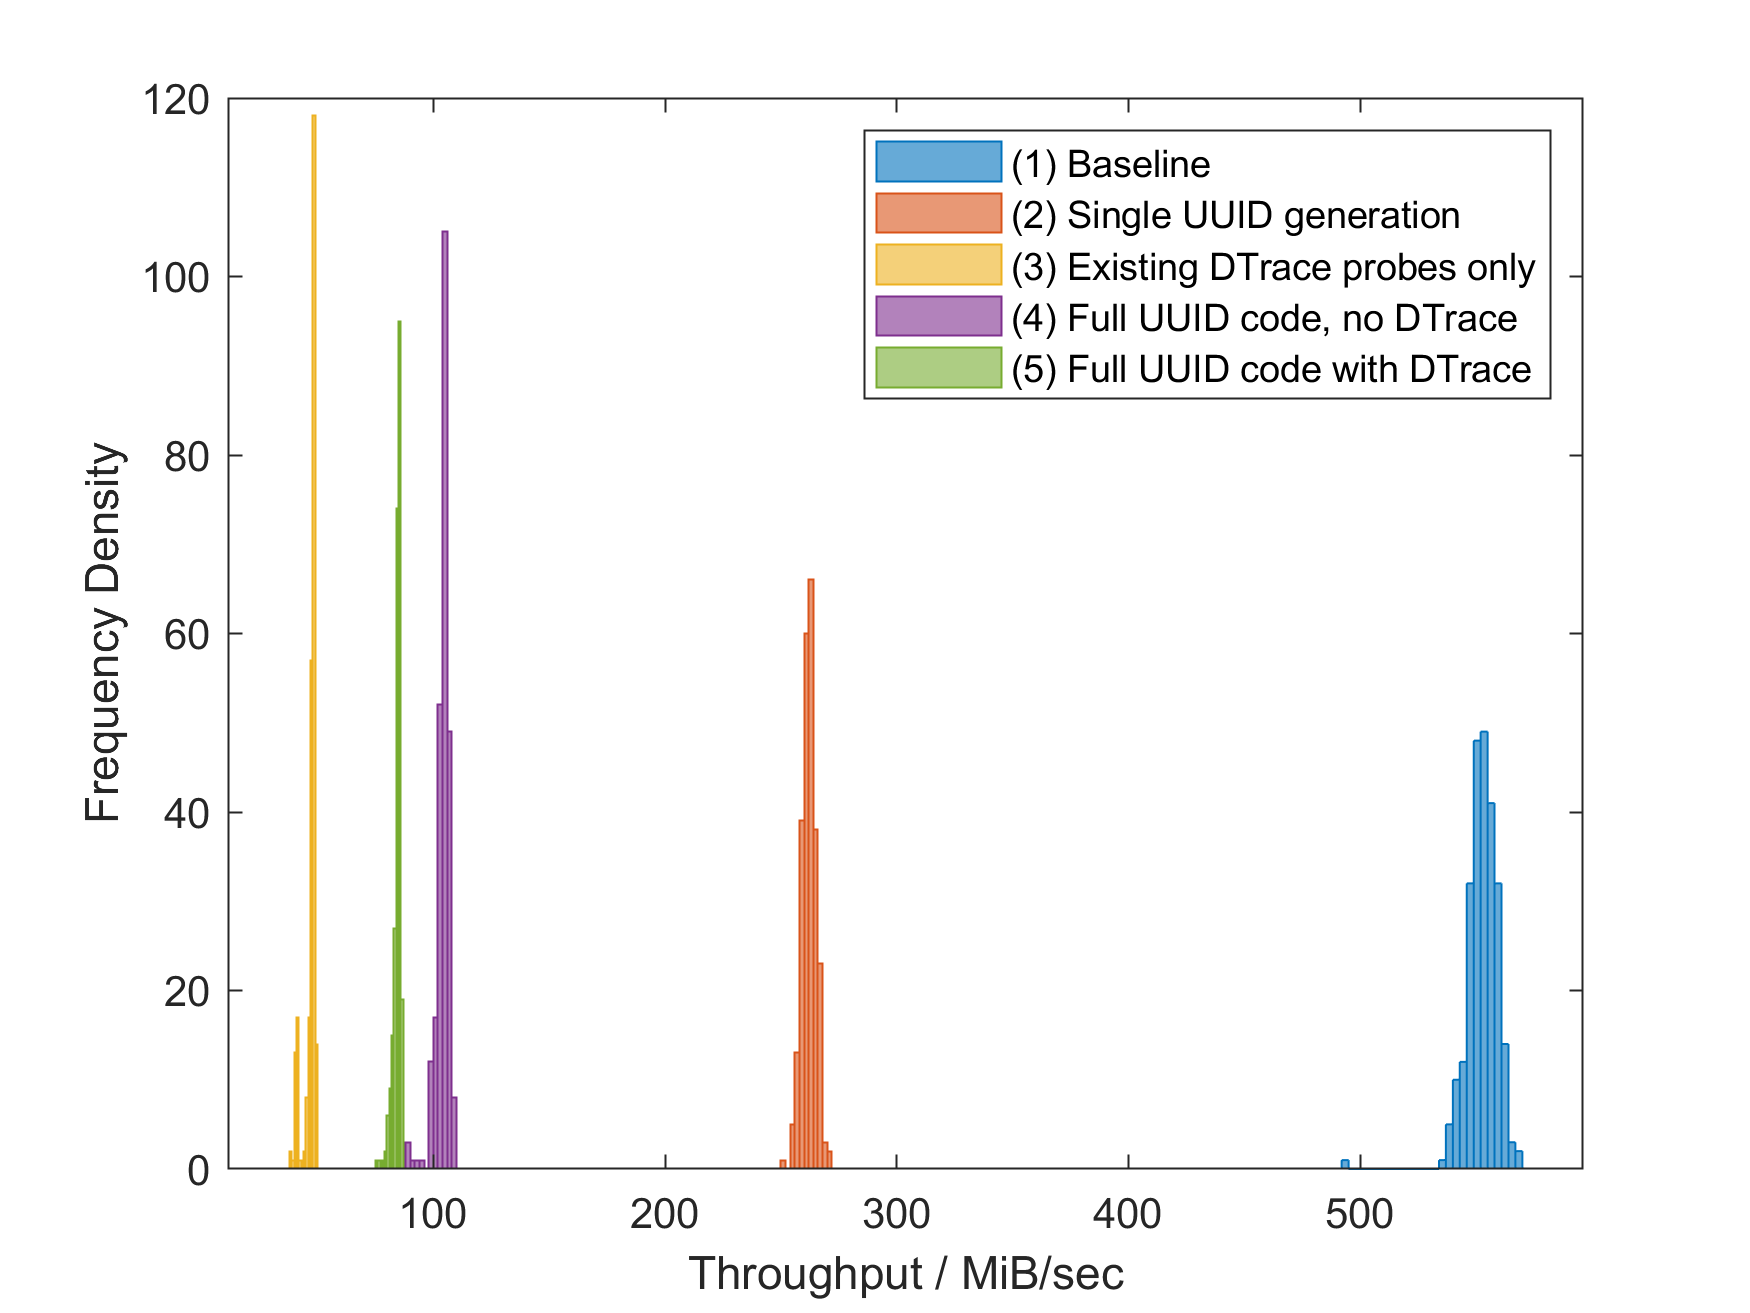
\includegraphics[width=0.9\linewidth]{include/ipc-mtu1500.png}
			\caption{Distributions using the standard Ethernet MTU of 1500 bytes.}
			\label{fig:ipc-eval-1500}
		\end{subfigure}
		\begin{subfigure}{\linewidth}
			\centering
			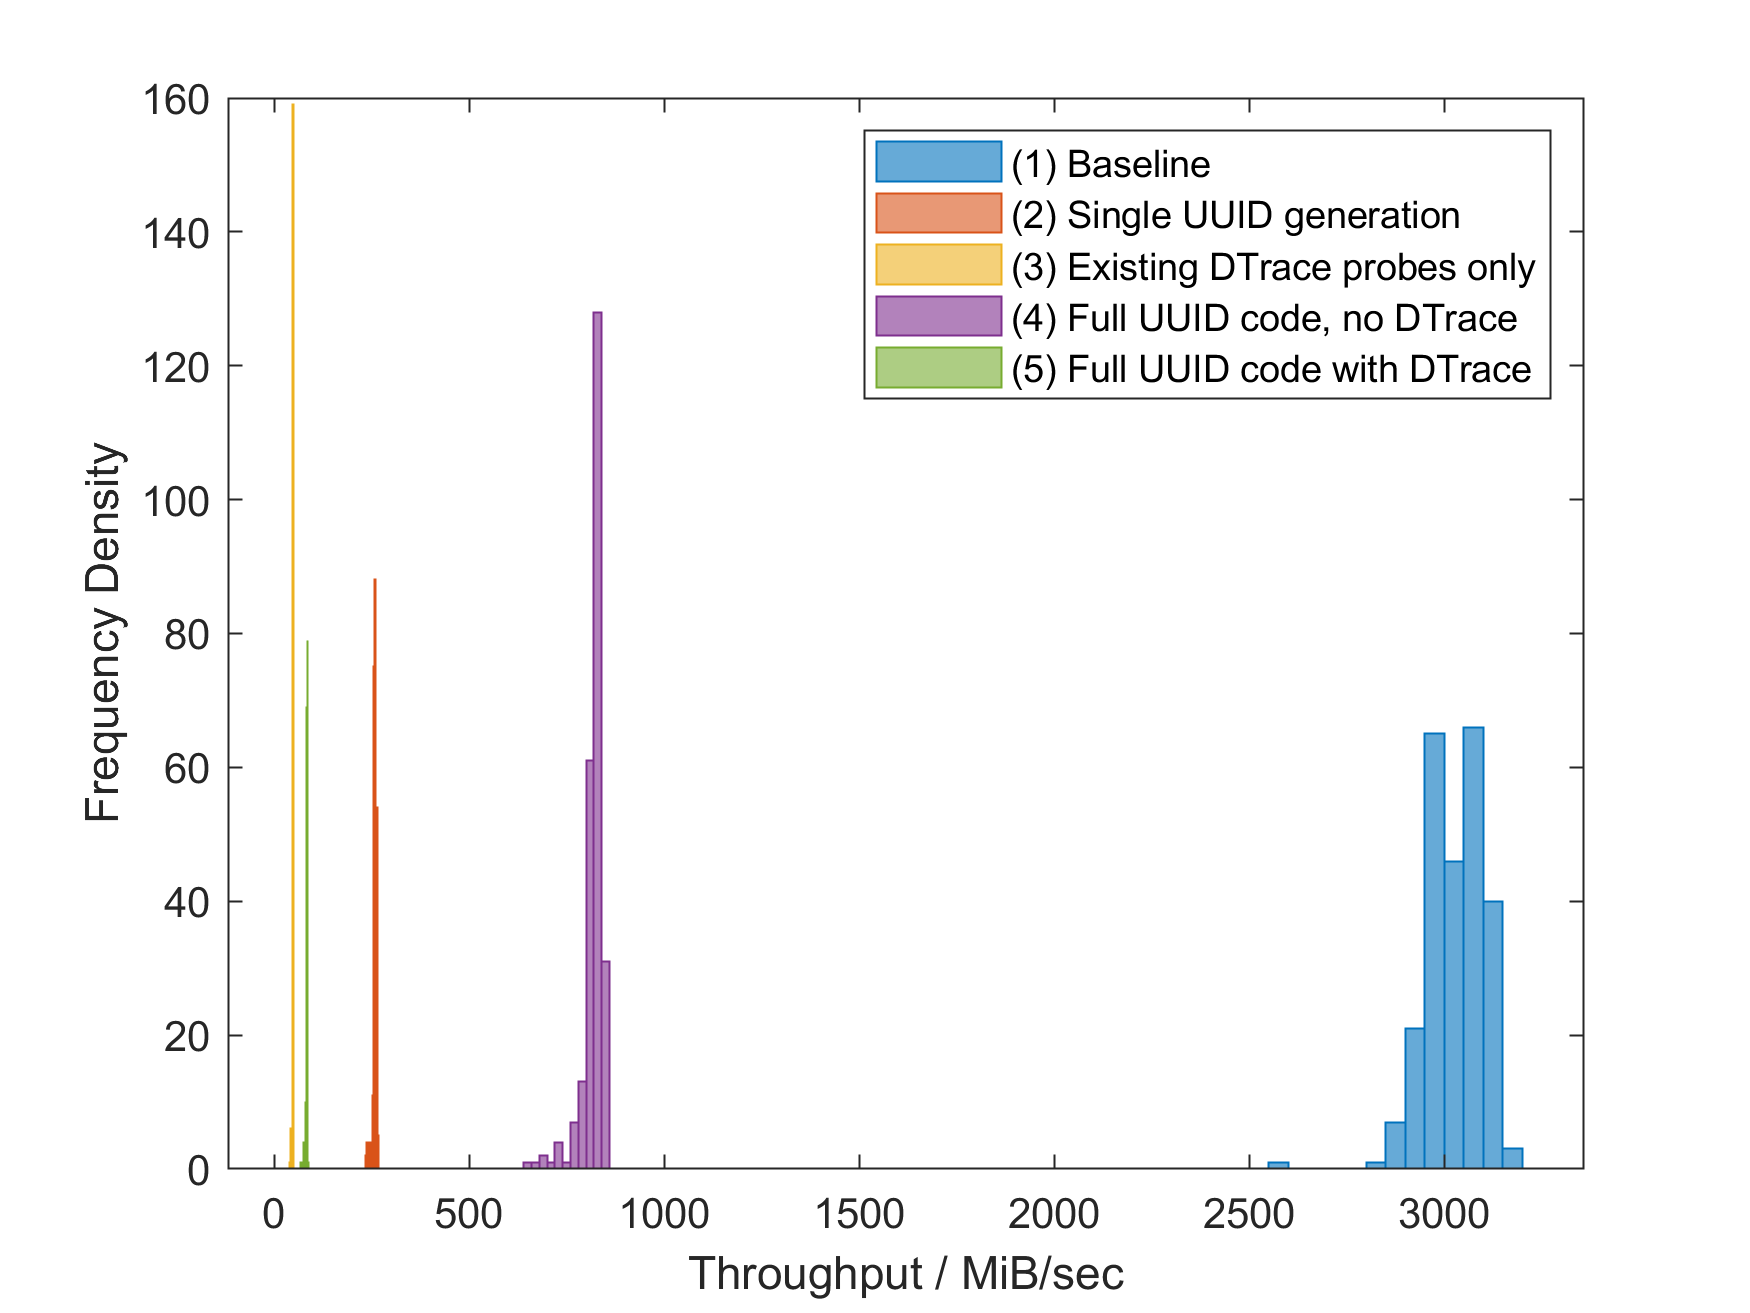
\includegraphics[width=0.9\linewidth]{include/ipc-mtu16k.png}
			\caption{Distributions using my system's default MTU of 16k bytes.}
			\label{fig:ipc-eval-16k}
		\end{subfigure}
		\caption{A pair of histogram plots generated from the benchmark data I collected with the two chosen MTU sizes, to assess the additive effect of each code component.}
		\label{fig:ipc-eval}
	\end{figure}

	In \figurename{ \ref{fig:ipc-eval-1500}}, we see that in all 5 scenarios the distribution of the throughput measurements appears close to a Gaussian distribution, although the list of coefficients of variation in \tablename{ \ref{fig:ipc-table}} shows that some of these distributions differ in scale. With a larger MTU of 16kbytes, however, it is clear that there are some differences in the distributions of the measurements from the histogram in \figurename{ \ref{fig:ipc-eval-16k}} simply by inspecting the shape. The distributions get particularly narrow in the later scenarios, which can also be seen numerically from the variance figures.
	
	\subsection{Analysis \& Conclusions}
	
	As expected, network throughput was lower when using UUID tagging and/or DTrace probes in the kernel in general, but it is particularly interesting to note that scenario 3, in which I simply used existing probes which are defined in a similar way to those I created in this project, had the lowest throughput for both MTU sizes. Perhaps this indicates that the complexity of the DTrace probes is more important than their number (since the full project code certainly has more enabled probes than scenario 3), as the built-in probes have relatively complex argument transformations to be performed in DTrace.
	
	At first glance, the effect of the project's code on system throughput looks to be very significant, as the code reduced throughput to just 2.8\% of its original value with a 16kbyte MTU, though with a 1500 byte MTU this rose to 15.2\%, a marked improvement. Despite these uninspiring figures, I argue that in normal use performance has not in fact been degraded, since these figures measured the maximum possible throughput on my machine. With the full project code enabled, both MTU values had a throughput measurement of 84MiB/sec, which equates to 672Mib/sec, and it is certainly very rare for a consumer PC to be able to saturate such a link speed under normal usage. Clearly the additional code in use will have implications for power consumption, but this was not a major concern in this project.
	
	Based on the analysis above where I argue that the achieved throughput when the project is in use is still sufficient for the type of computer the benchmarks were run on, I claim that the project has satisfied the second part of its success criterion, which relates to the performance impact of the project.
	
	\subsection{Moving work into DTrace}
	\label{sec:dtrace-iteration}
	
	It is particularly apparent from \figurename{ \ref{fig:ipc-eval-1500}} that little performance difference was observed between scenarios 4 and 5, the principle difference between which is the enabling of the project's new DTrace probes. This may suggest that the disabled DTrace probes are incurring too high a cost to normal execution; keeping these costs as low as possible was a design goal of DTrace\cite{Gregg-DTrace}.
	
	The obvious unnecessary additional cost being incurred by almost all added probes is that they have to extract a packet's UUID in order to pass this to the probe. Recall that UUIDs are part of a set of so-called \texttt{tags} attached to a particular \verb|mbuf|, and so finding the appropriate tag is performed in the kernel using \verb|m_tag_locate|. Currently this is being called for every packet which has a UUID, even if the probes are disabled, and so providing a copy of this function in DTrace's D language would allow the disabled probe effect to be reduced to near zero again. Unfortunately this is not a trivial option as it requires a loop over a linked list, and iteration primitives to support such a loop are not provided in the D language.
	
	Iteration primitives are not provided by the D language as DTrace also puts significant emphasis on not affecting the code it instruments, in this case the kernel, providing guarantees on memory access and so forth. A lack of support for iteration guarantees by construction that code written in the language cannot form an infinite loop and so cannot affect the kernel's behaviour in that way. As further work, I propose instead modifying the D language to support a general form of bounded iteration, which could then be used by a copy of \verb|m_tag_locate|, in order that we may still provide a guarantee that all D code will terminate whilst increasing the expressiveness of the language.
	
	\section{Functionality of example application}
	
	The example application which I have produced fulfils the requirements of extension number one in my project proposal, which was to present collected data in a user-friendly format, as well as demonstrating that the project fulfils the first part of its success criterion, namely that it collects the data in the first place. The Web-based tool allows any computer with a Web browser to be used as a client for analysis, and therefore can include non-FreeBSD systems if required.
	
	\begin{figure}
		\centering
		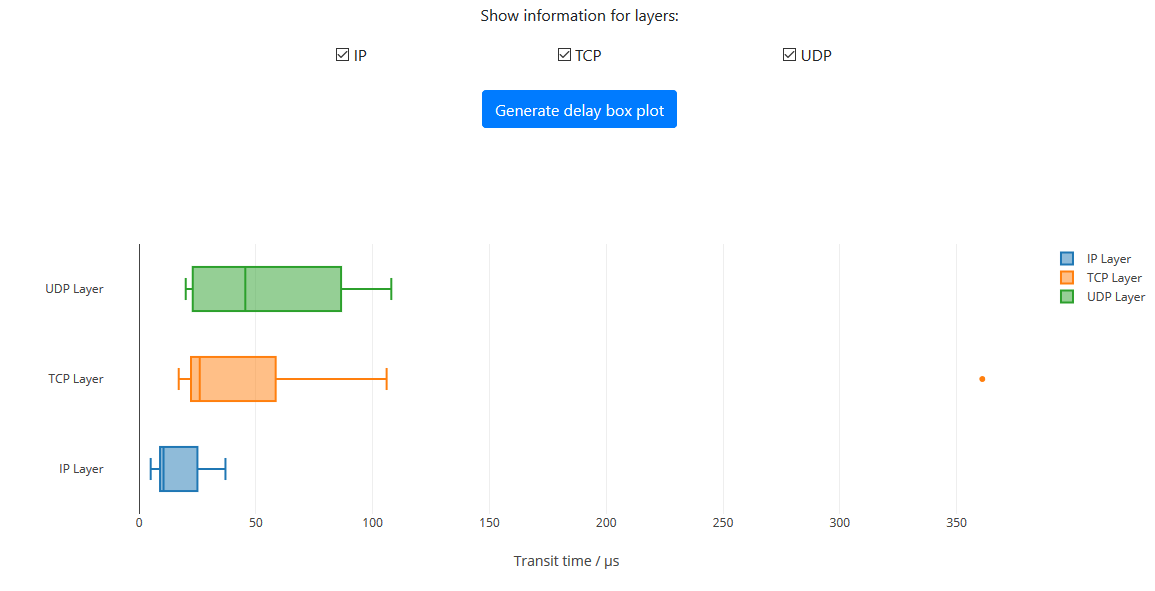
\includegraphics[width=\linewidth]{include/ui-timing-box.png}
		\caption{The application can display statistical information about the time packets have spent in each layer of the network stack. It queries the backend application to find what layers it understands on the current system, and then provides options to the user for them to request information about any layers they are interested in.}
		\label{fig:ui-timing-box}
	\end{figure}

	\begin{figure}[b]
		\centering
		\caption{The application provides a heatmap of the kernel address space, showing which kernel memory addresses are most commonly used to store packet data. Clicking on a heatmap cell draws a new `zoomed in' heatmap of the data which fits logically within that cell.}
		\label{fig:ui-heatmap}
	\end{figure}
	
	\chapter{Conclusion}
	
	The goals of this project were to provide metadata collection tools for network packets by tracking individual packets as they flow through the network stack of the FreeBSD kernel, allowing timing and other information to be collected and queried at a later stage. The provision of UUID tagging in combination with new DTrace kernel probes has facilitated this data collection, and I have evaluated the performance impact of my project as a whole to find that it is acceptable. This means that the project's success criterion, as defined on page 3 of the attached project proposal, has been met.
	
	In addition to the core project's success, I have also completed the work required for extension number one in producing a user application to analyse the data collected from the running kernel and presenting this in a user-friendly and interactive format.
	
	\section{Further Work}
	
	My principal proposition for further work is to add provision for bounded iteration to DTrace's D language, as I outlined in Section \ref{sec:dtrace-iteration}.
	
	Additionally, it is clear that I chose not to use any automated static analysis tools in my work on existing kernel code as part of the project. This decision was taken because I did not feel that any benefit would be gained from doing so in this case, as it would have taken me just as long to familiarise myself with what I was looking for within the kernel code and set the tools up to do this, as it did for me to inspect the source manually. Now that I have a better understanding of the kernel code in question, in future I would consider more seriously the possibility of using such tools.
	
	%%%%%%%%%%%%%%%%%%%%%%%%%%%%%%%%%%%%%%%%%%%%%%%%%%%%%%%%%%%%%%%%%%%%%
	% the bibliography
	\addcontentsline{toc}{chapter}{Bibliography}
	\bibliographystyle{plain}
	\bibliography{refs}
	
	%%%%%%%%%%%%%%%%%%%%%%%%%%%%%%%%%%%%%%%%%%%%%%%%%%%%%%%%%%%%%%%%%%%%%
	% the appendices
	\begin{appendices}
		\chapter{IPC Benchmark shell script}
		\label{appendix:IPC}
		
		The following shell script was used to execute the IPC benchmark 100 times to gather data on the throughput effects of the different UUID algorithms.
		
		\begin{verbatim}
		#!/bin/csh
		
		# First argument is ipc executable
		set ipc=$1
		# Second argument is csv file to output to
		set csv=$2
		
		# Overwrite any existing file with the header
		echo "Measured transfer rate" > $csv
		
		@ n = 0
		# Repeat the benchmark 100 times
		while ($n < 100)
		    # Allow the system to calm down before running benchmark
		    sleep 2
		    # 16GiB transfer is found to put the system under significant
		    # load for about 10 seconds, on my machine
		    $ipc -i tcp -t 17179869184 2proc | awk '{print $1}' >> $csv
		    @ n += 1
		end
		\end{verbatim}
	\end{appendices}
	
	
	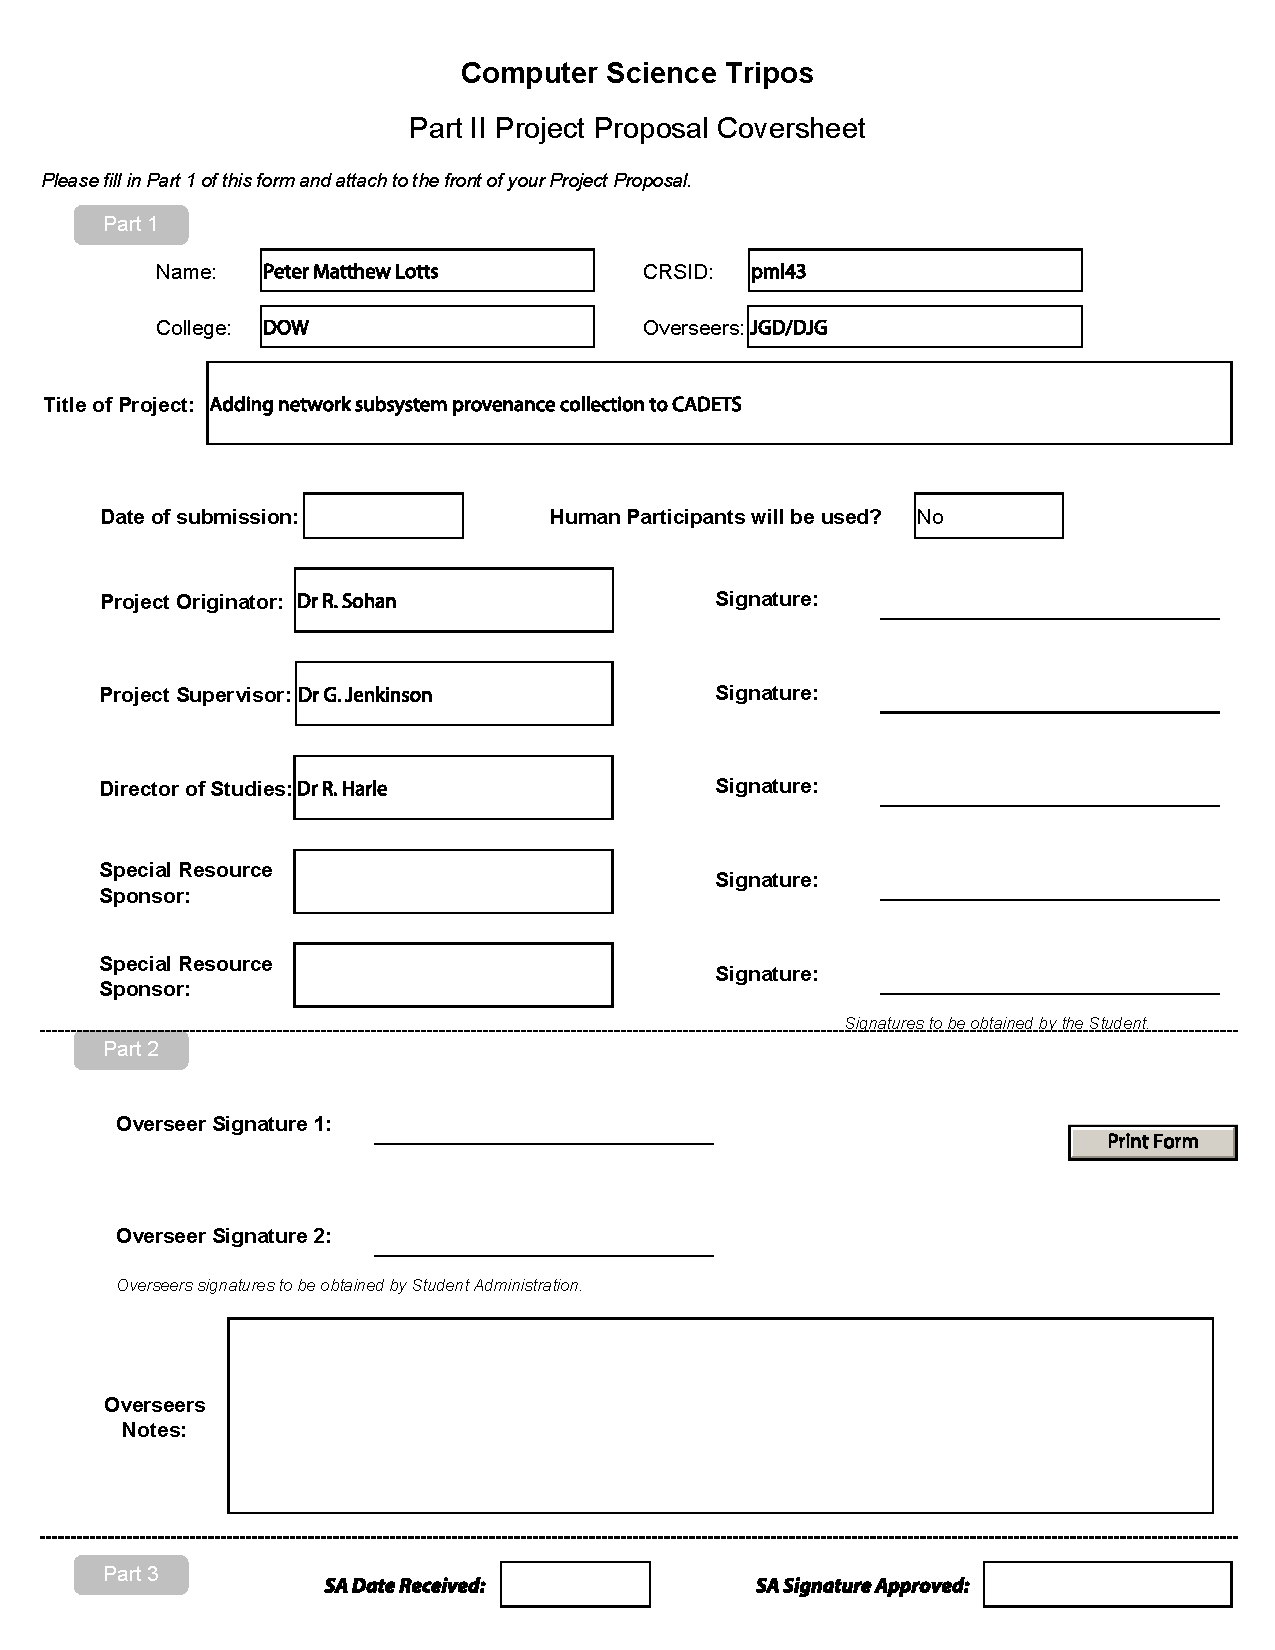
\includepdf{include/Project-Proposal-Cover-Sheet.pdf}
	\includepdf[pages={2-}]{include/Project-Proposal.pdf}
	
	
\end{document}
